The prototype developed intends to be integrated with a PCB (printed circuit board) currently being developed by the Boutelle group. The PCB consists of five potentiometric channels, allowing for the measurement of potassium ion concentration and four amperometric channels to allow for glucose and lactate concentration measurements. The potentiometric readings are amplified using an instrumental amplifier (IA), and the amperometric readings are amplified using a transimpedance amplifier (TIA), which also converts the inputted current to a voltage signal. An ADS1298, which is a 24-bit resolution analogue-to-digital converter (ADC), receives the input measurements simultaneously and discretises and further amplifies the signals \cite{TexasInstruments2010}. An ATmega328p microcontroller is used and the PCB allows for both SPI (serial peripheral interface) and UART (universal asynchronous receiver-transmitter) data transmission capabilities. The PCB functionality is summarised in the block diagram in Figure~\ref{fig: PCB block diagram}.

\begin{figure}[h!]
\centering
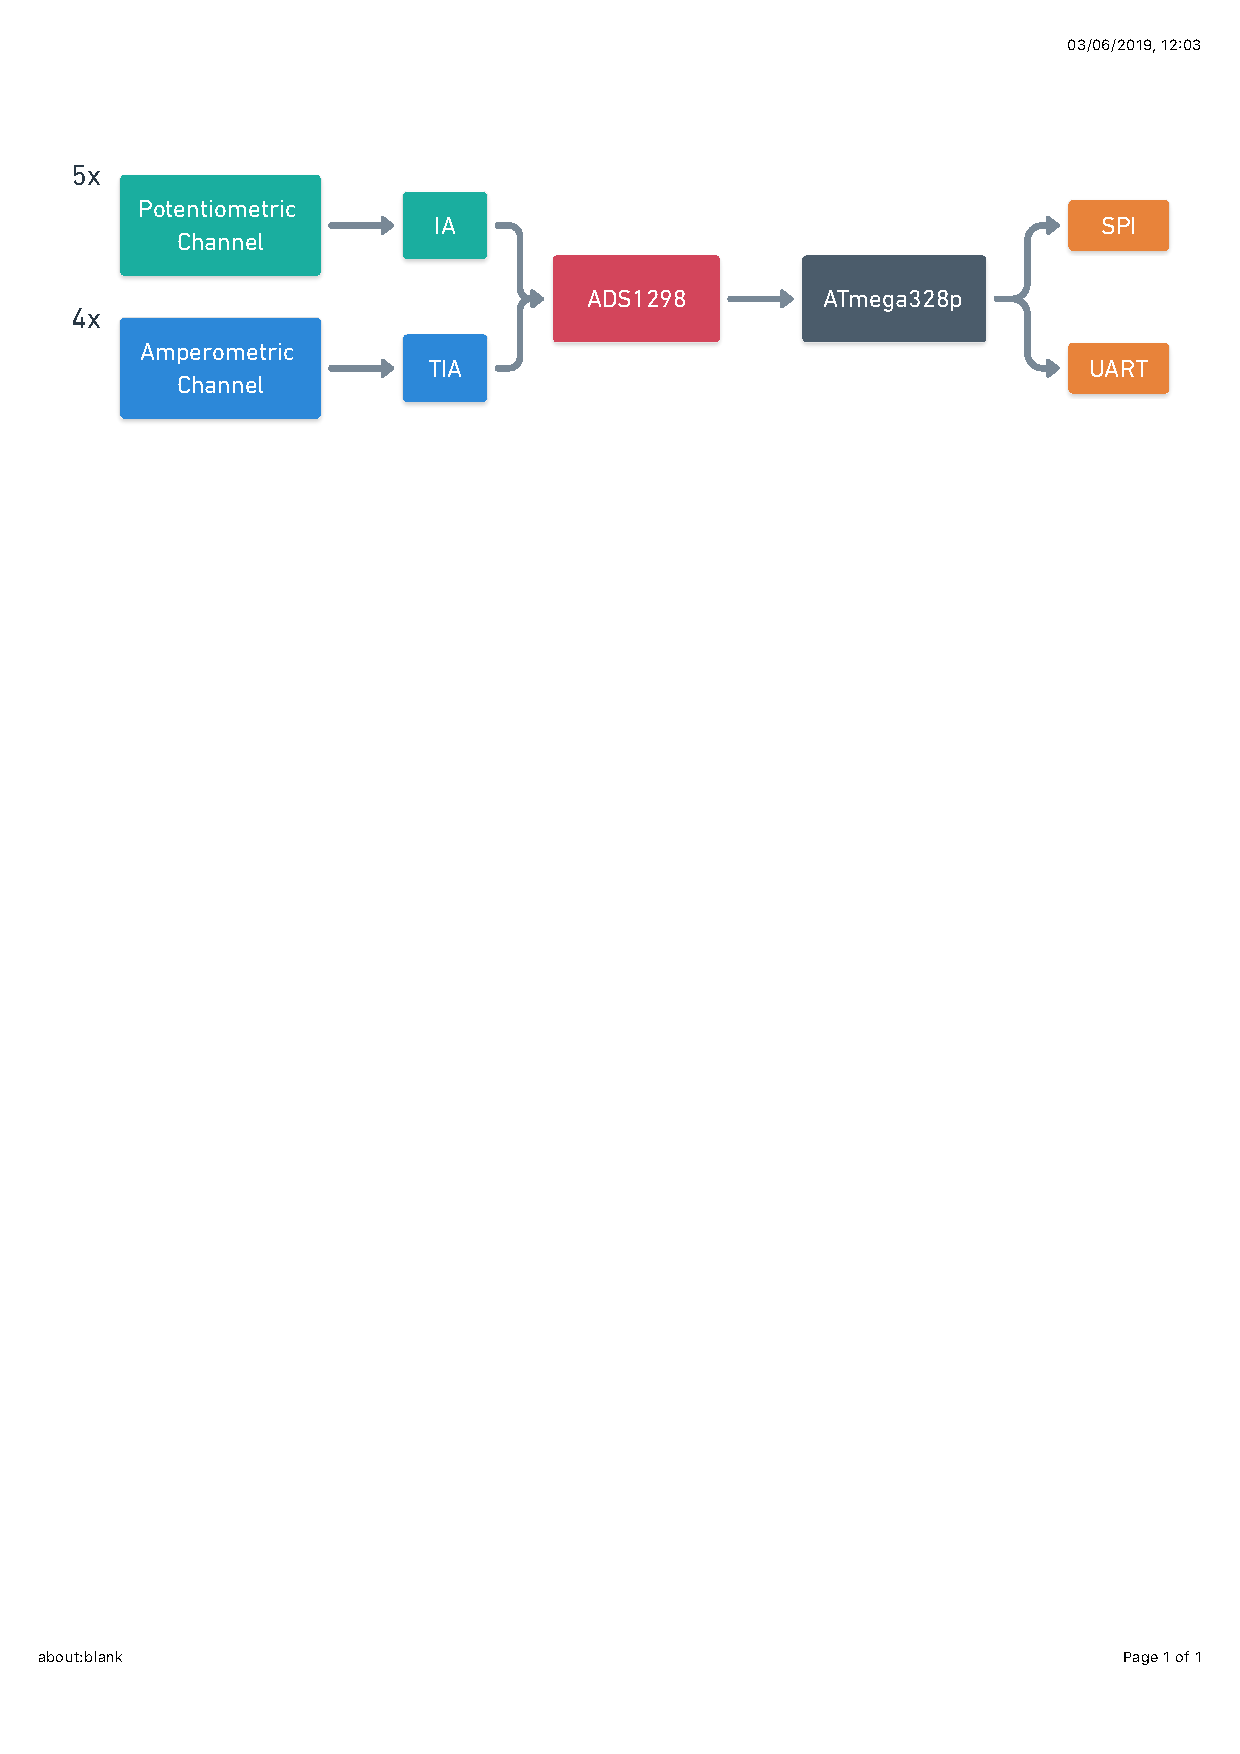
\includegraphics[trim={0cm 20.5cm 0.5cm  2.9cm}, clip, width=1\textwidth]{./figures/CircuitBlockDiagram.pdf}
\captionsetup{justification=centering}
\caption{Block Diagram of the PCB being developed by the Boutelle Group for continuous monitoring of TBI markers.}
\label{fig: PCB block diagram}
\end{figure}

\begin{figure}[b!]
\centering
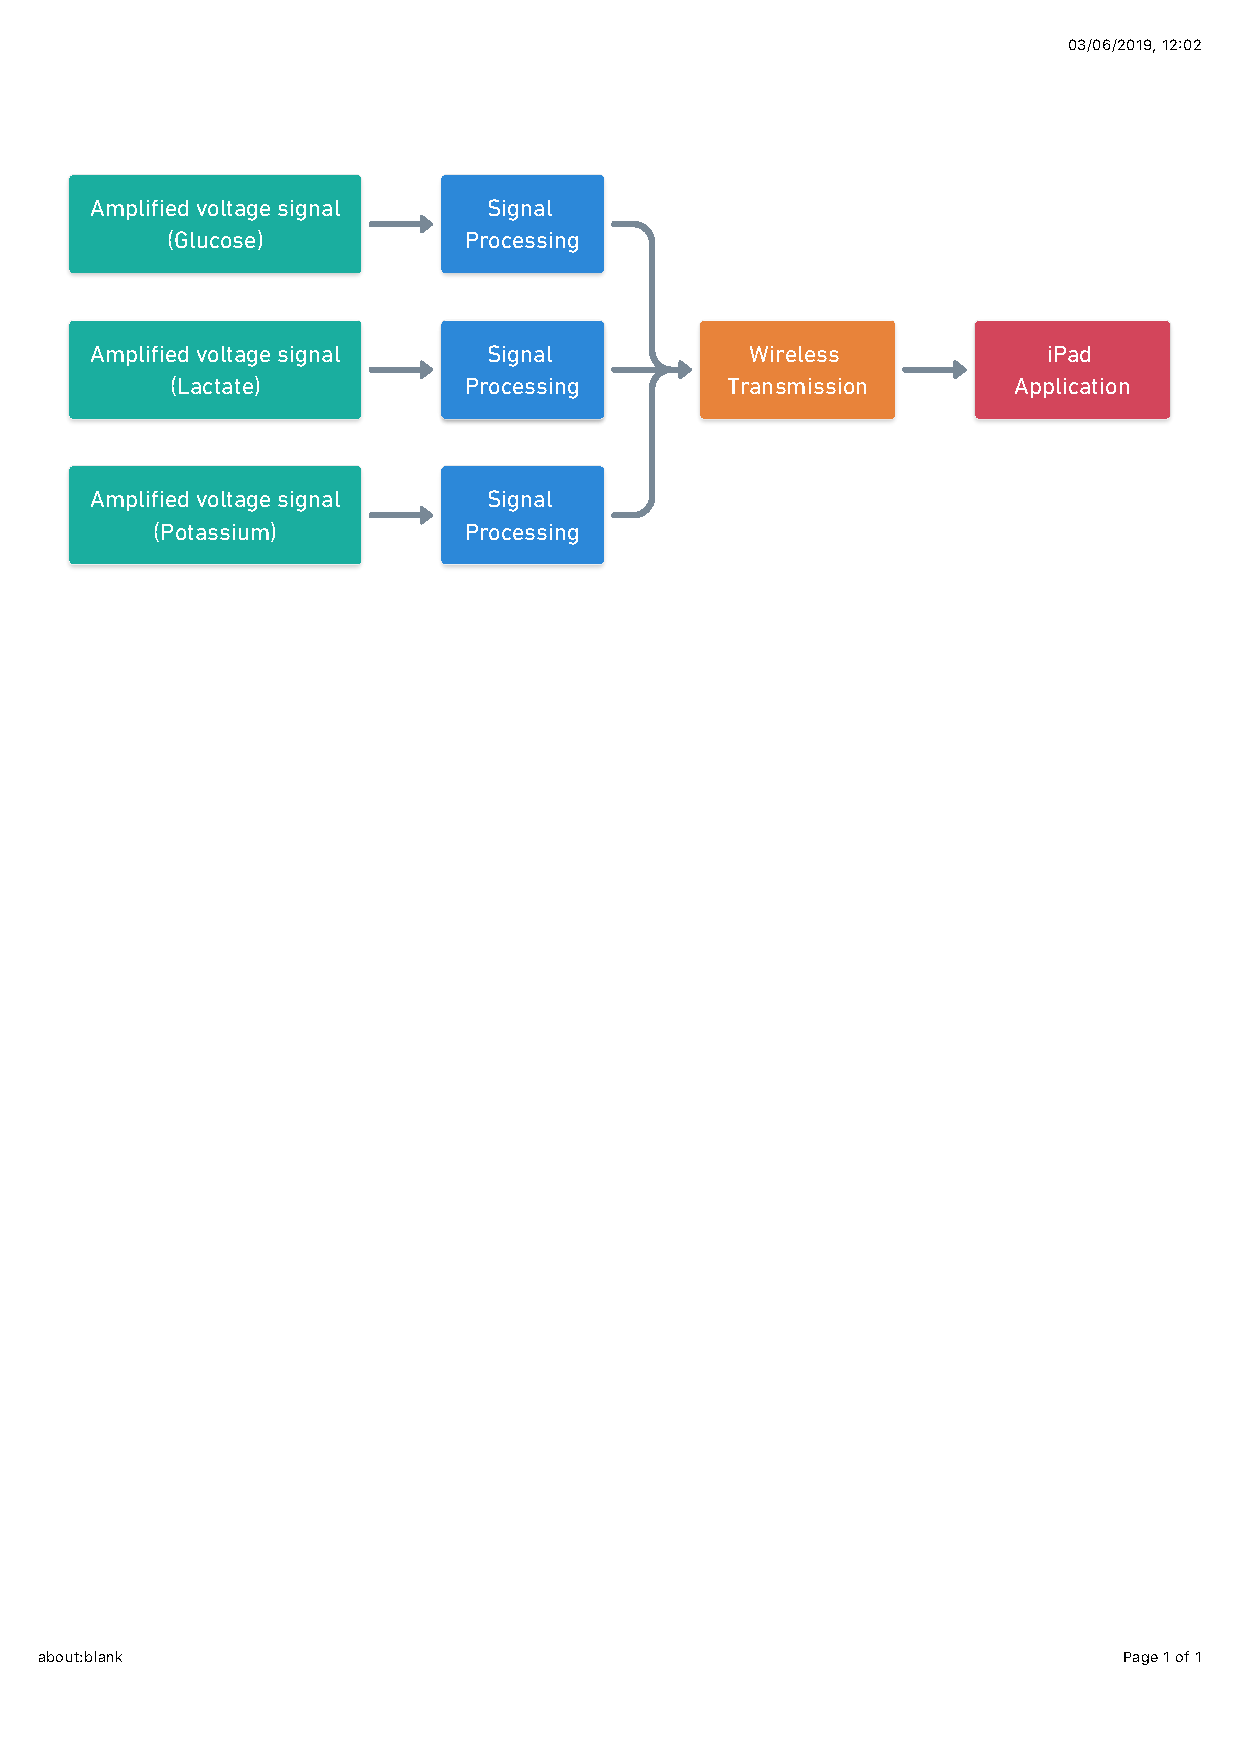
\includegraphics[trim={0cm 19.5cm 0.5cm  2.5cm}, clip, width=1\textwidth]{./figures/Flowchart.pdf}
\captionsetup{justification=centering}
\caption{Flowchart of the key elements in the prototype system.}
\label{fig: flowchart}
\end{figure}

I have developed a prototype that simplifies the hardware of the PCB. The prototype receives three amplified voltage signals, corresponding to glucose, lactate and potassium, so it continues on from the PCB block diagram after the ADS1298. In addition to the hardware, the prototype includes signal processing, wireless transmission of the data, and the development of an iPad application, as shown in the flowchart in Figure~\ref{fig: flowchart}. The prototype provides a simplified platform for the wireless transmission to be developed. The prototype can then be integrated with the research group's PCB, which is due summer 2019.



\subsection{Hardware}
The hardware for the prototype consists of an Arduino Nano and an Adafruit Bluefruit LE SPI Friend, as shown in Figure~\ref{fig: breadboard}. The Arduino Nano was chosen as a suitable microcontroller for prototyping and mimicking the PCB as it also contains an ATmega328p microcontroller and has an inbuilt ADC. The ADC is only 10-bit, so it has poorer resolution than the ADS1298. However, the Arduino is simple to programme due to the IDE and libraries available, making it suitable for prototyping.

\begin{figure}[H]
\centering
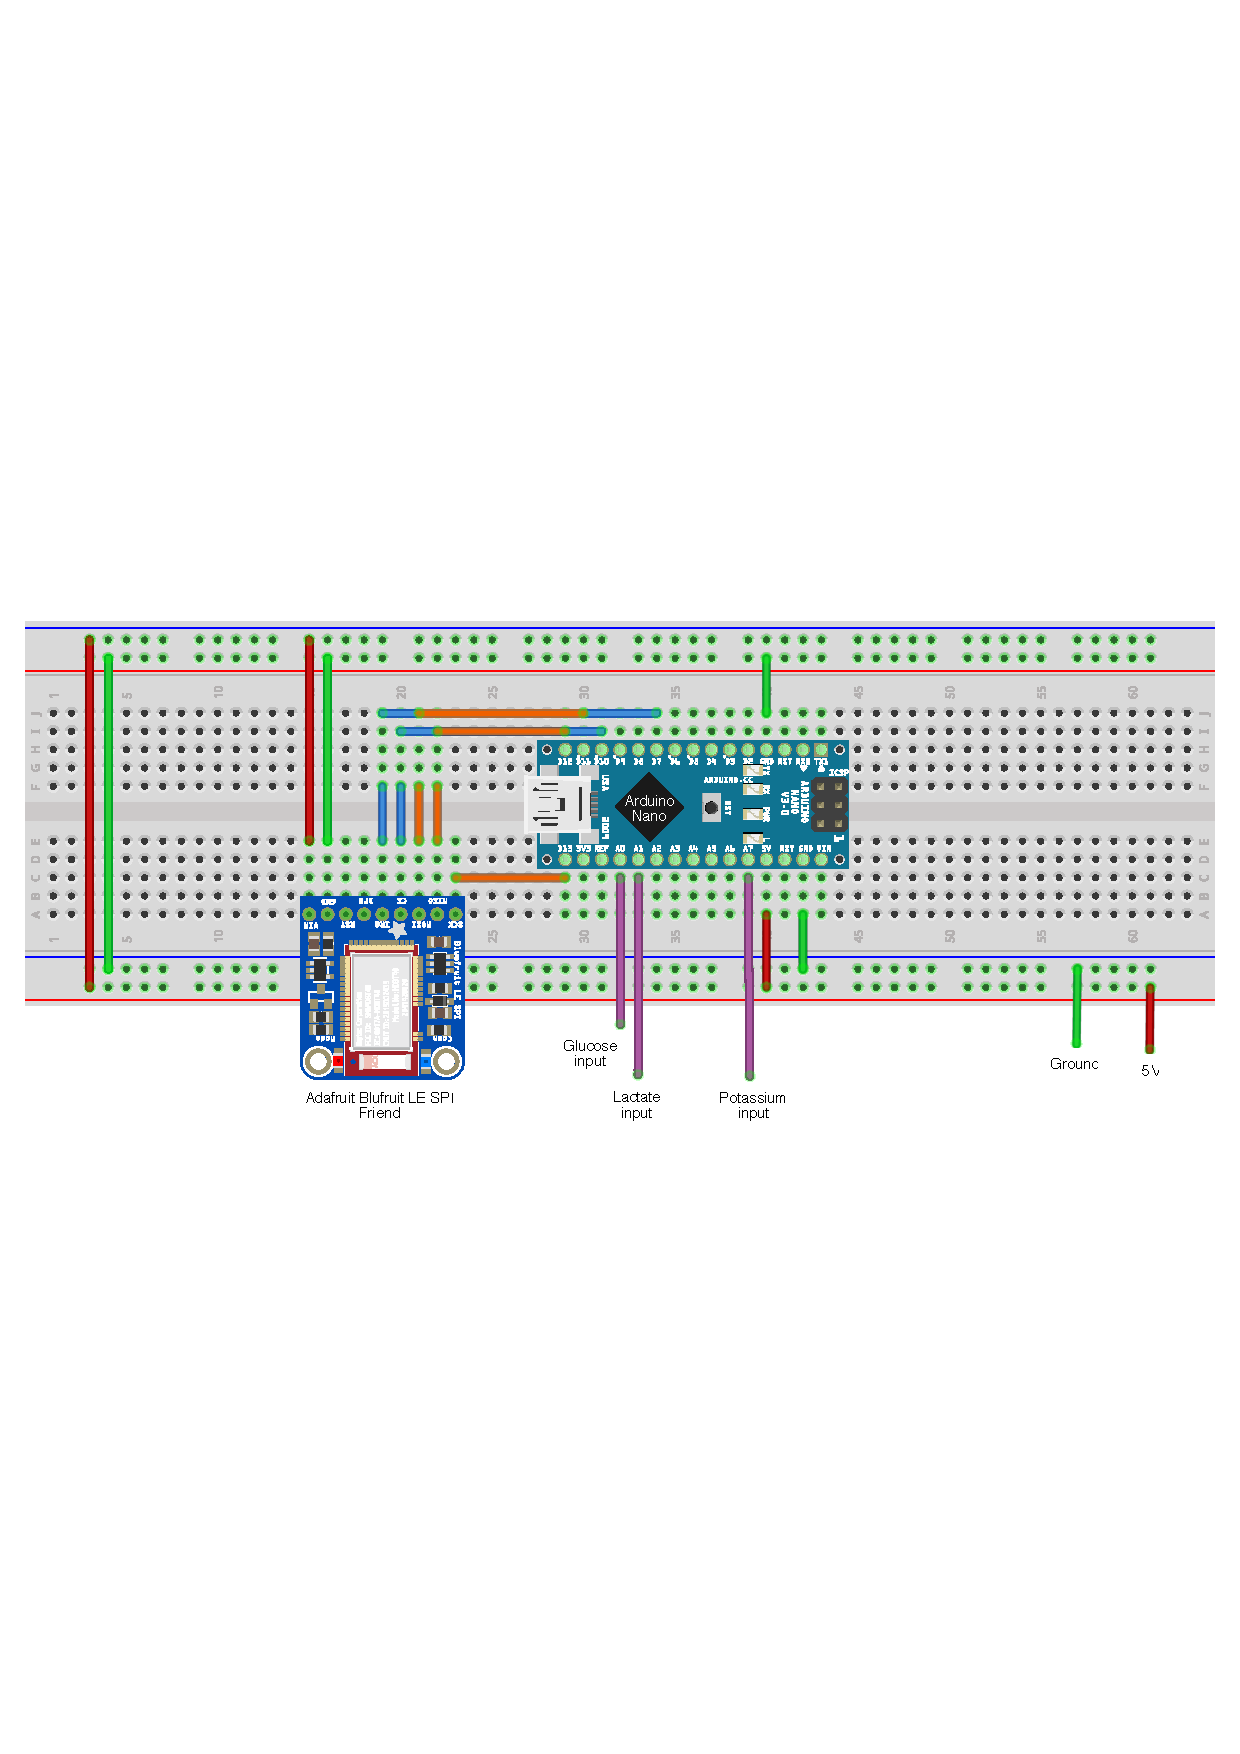
\includegraphics[trim={0cm 10.5cm 0cm  10cm}, clip, width=1\textwidth]{./figures/Breadboard2.pdf}
\captionsetup{justification=centering}
\caption{Prototype assembled on breadboard.}
\label{fig: breadboard}
\end{figure}

The Arduino Nano receives three input voltage signals ranging from 0V to 5V at the analogue pins A0, A1, and A7. These input pins correspond to glucose, lactate, and potassium. The signals are discretised by the Arduino's inbuilt ADC. The Arduino records the time at which each signal is read, along with the value of the signal, and processes the recordings before passing them to the Bluefruit module.




\subsection{Firmware}
The Arduino Nano is encoded to sample and process the three input signals received, then to control the Bluefruit to wirelessly transmit the signals via Bluetooth low energy (BLE). The algorithm encoded in the Arduino is described in Figure~\ref{fig: psuedocode}. The code for my project can be found in Appendix~\ref{appendix: a}.

\begin{figure}[t!]
\centering
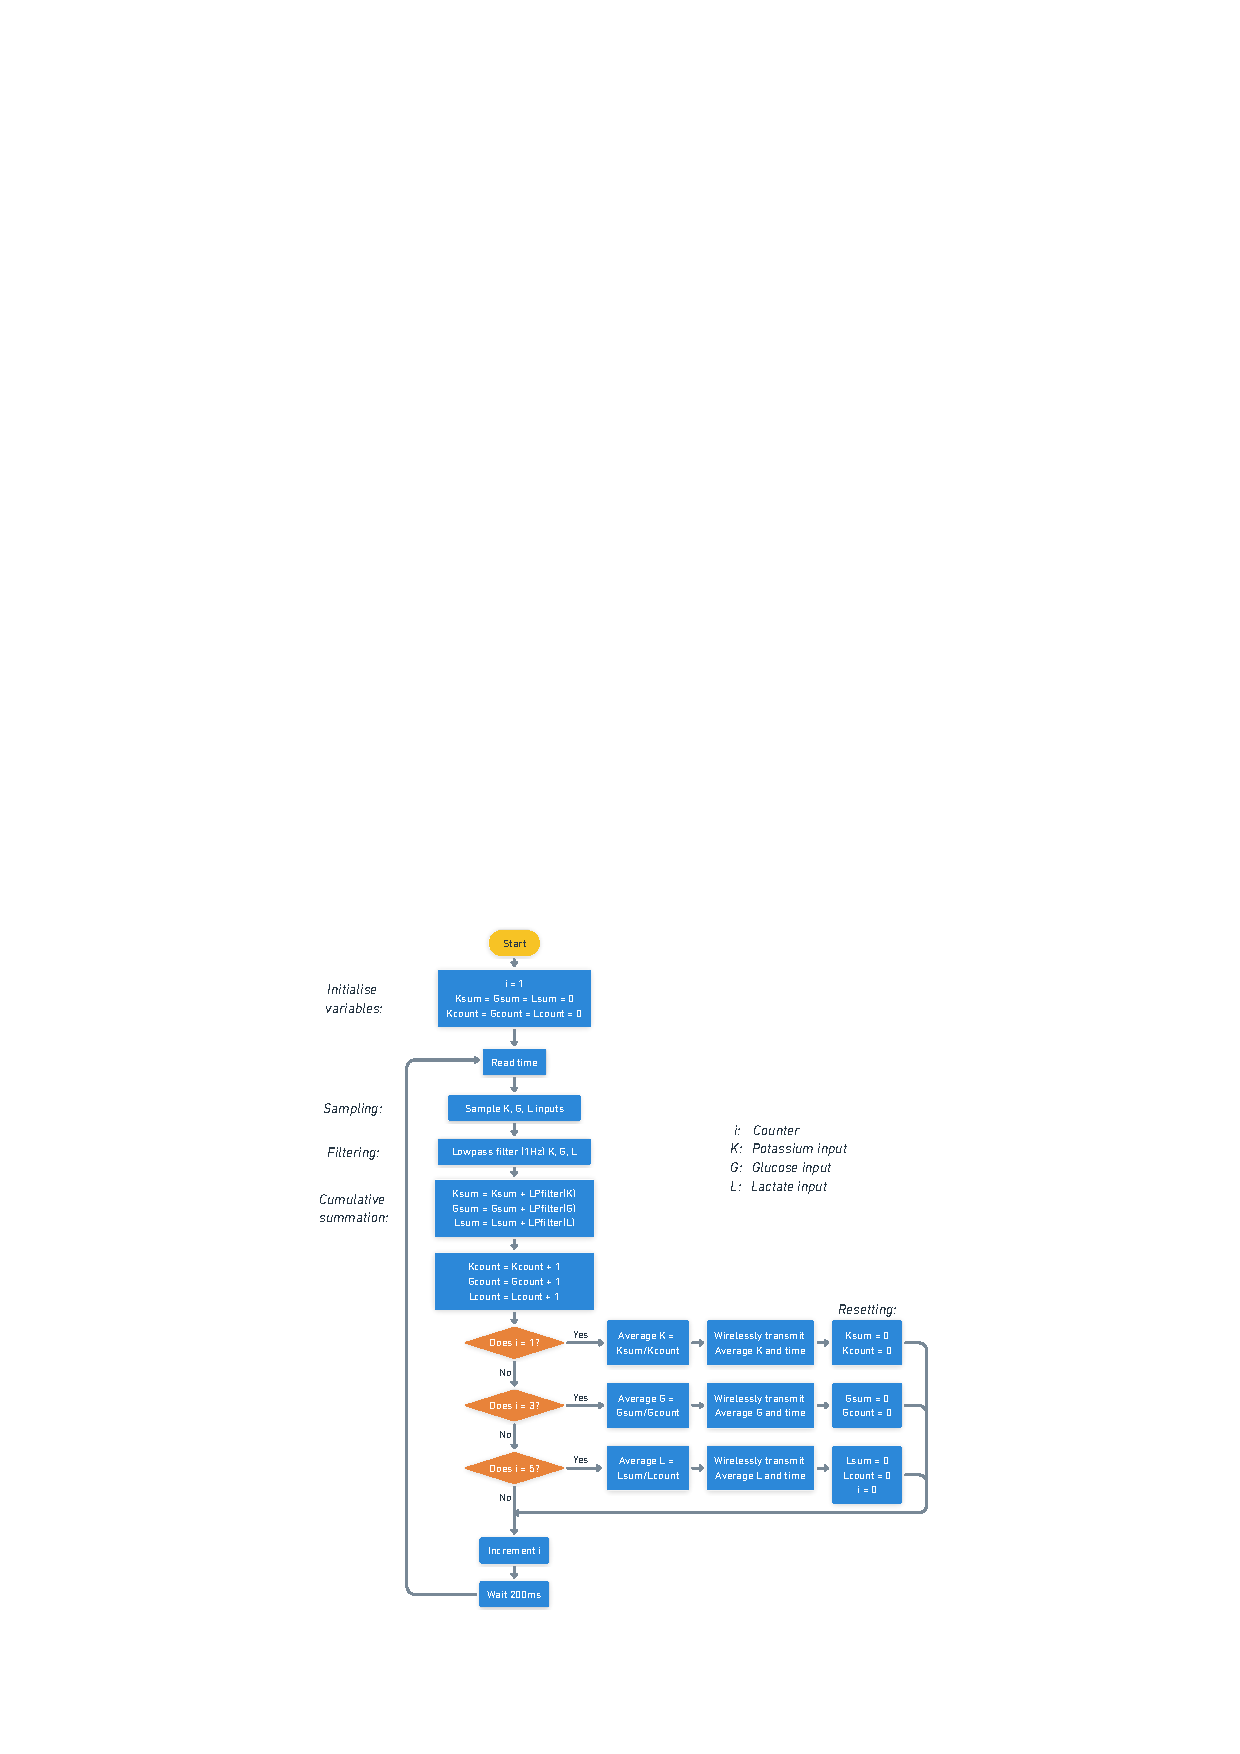
\includegraphics[trim={0cm 0cm 0cm  0cm}, clip, width=1\textwidth]{./figures/psuedocode.pdf}
\captionsetup{justification=centering}
\caption{Flowchart of algorithm encoded in Arduino Nano.}
\label{fig: psuedocode}
\end{figure}


\subsubsection{Signal Processing}
Every 200ms the Arduino reads the input signals at the A0, A1 and A7 pins and records the time (in milliseconds since the Arduino was connected to power) at which sampling occurred. Each input signal received by the Arduino is filtered with a low-pass filter with a cut off frequency of 1Hz. This cut off frequency was chosen because the events indicating an SD occur over a long time frame, as shown in Figure~\ref{fig: SD}, hence the changes occur slowly and at low frequency. The low pass filter attenuates high frequency components that may arise from noise or patient movement, allowing for a cleaner signal to be obtained.

For every five samples of data recorded (1s period) the mean voltage is calculated for each electrochemical signal. This averaging methods allows large deviations and spikes to be smoothed, thereby reducing the effect of noise on the outputted data. This averaged value is then transmitted to the iPad app, and the raw input readings are discarded.



\subsubsection{Wireless Transmission}
BLE and ZigBee are both popular wireless data transmission options for IoT projects. Table~\ref{table:BLE vs ZigBee} summarises the differences between BLE and ZigBee. For this project, BLE is the most suitable option as it offers more efficient data transfer, shown by the lower latency time and higher throughput, consumes less power, and is compatible with iOS. A disadvantage of BLE is that it has a shorter range than ZigBee, however the range is sufficient for this project since the patient will remain close to the iPad that will receive the transmitted signals.

\begin{table}[h!]
\centering
\begin{tabular}{||c c||} 
 \hline
 BLE & ZigBee \\ [0.5ex] 
 \hline\hline
 Range: 77m & Range: 291m \\
 Data rate: 1Mbps bursts & Data rate: 250kbps \\ 
 PAN (personal area network) & LAN (local area network) \\
 Throughput: 0.27Mbps & Throughput: 0.03Mbps \\
 Latency: 3--6ms & Latency: 15ms \\
 Sleeps between bursts $\rightarrow$ uses less power & No sleep functionality \\
 Supported on most OSs including iOS & Not supported on most OSs \\
 \hline
\end{tabular}
\caption{BLE vs. ZigBee \cite{Ray2015, Christiano}.}
\label{table:BLE vs ZigBee}
\end{table}

Adafruit provide a variety of Bluetooth low energy modules that are compatible with Arduino, and they provide a library that can be used with the Arduino IDE: Adafruit\_BluefruitLE\_nRF51. Adafruit also provide an iOS app to test the Bluetooth module and view the received signals which is useful to test intermittent stages in the development process. Whilst the PCB currently being developed allows for both SPI and UART data transmission, SPI was the chosen mode of data transfer for the prototype as SPI utilises synchronous transmission, meaning that data is sent in chunks with a constant time interval \cite{teachcomputerscience2018}. Furthermore, the SPI module is smaller than the equivalent UART module, so allows the final design of the PCB to be made smaller.

The Arduino Nano has inbuilt SPI pins: D11 is MOSI (Master Out/Slave In), D12 is MISO (Master In/Slave Out) and D13 is SCK (serial clock). These connect to the corresponding pins on the Bluefruit, shown by the orange connections in Figure~\ref{fig: breadboard}. The SPI CS (chip select) and IRQ (interrupt) pins have to be programmed onto the Arduino and are assigned as D10 and D7 respectively; blue wires show the connections to the Bluefruit.

The Adafruit Bluetooth library provides functions that allow for the transmission of data via BLE to a paired device. The limitation of transmission is that numbers are sent as strings, which requires more bytes than sending as an integer, and a maximum of 20 characters can be sent at a time \cite{Townsend2018} otherwise the data becomes fragmented. This means that the data from each input pin and the corresponding time of recording has to be wirelessly transmitted one at a time rather than all three sent simultaneously to prevent the risk of the data fragmenting. The data from each input pin is outputted in characters as:

\begin{align}
    \tt{OutputString = ID + Time + Voltage + ``\backslash n"}.
    \nonumber
\end{align}

The \textit{ID} at the beginning identifies which signal is being sent, i.e. G for glucose, and the newline character (\textit{$``\backslash$n"}) at the end concludes the string being transmitted. If both these identifiers are not present at these specific locations when received on the app, this indicates that the data is fragmented and the app will discard the data. 

Another limitation was observed when all three strings were periodically sent within a 200ms period. The data would initially be sent correctly but after a few minutes, the data would fragment. The Bluefruit struggled to send the data at a sufficient speed, which created a backlog of data that was responsible for the fragmentation. Eventually, the Bluetooth module would disconnect from the app. To prevent this, the three signals were periodically sent every 1s as highlighted in Figure~\ref{fig: psuedocode}. Since the electrochemical changes in the brain occur at low frequencies, a receiving rate of 1s on the app is sufficient for this application. 





\subsection{iPad Application}
The iPad app was written in Swift. The app layout is shown in Figure~\ref{fig: storyboard}. The three pages shown in section 3 of Figure~\ref{fig: storyboard} all have the same layout. Details of this layout can be seen clearly on the Potassium Ion Concentration page, and the pages Glucose Concentration and Lactate Concentration have the same features. 

\begin{figure}[p]
\centering
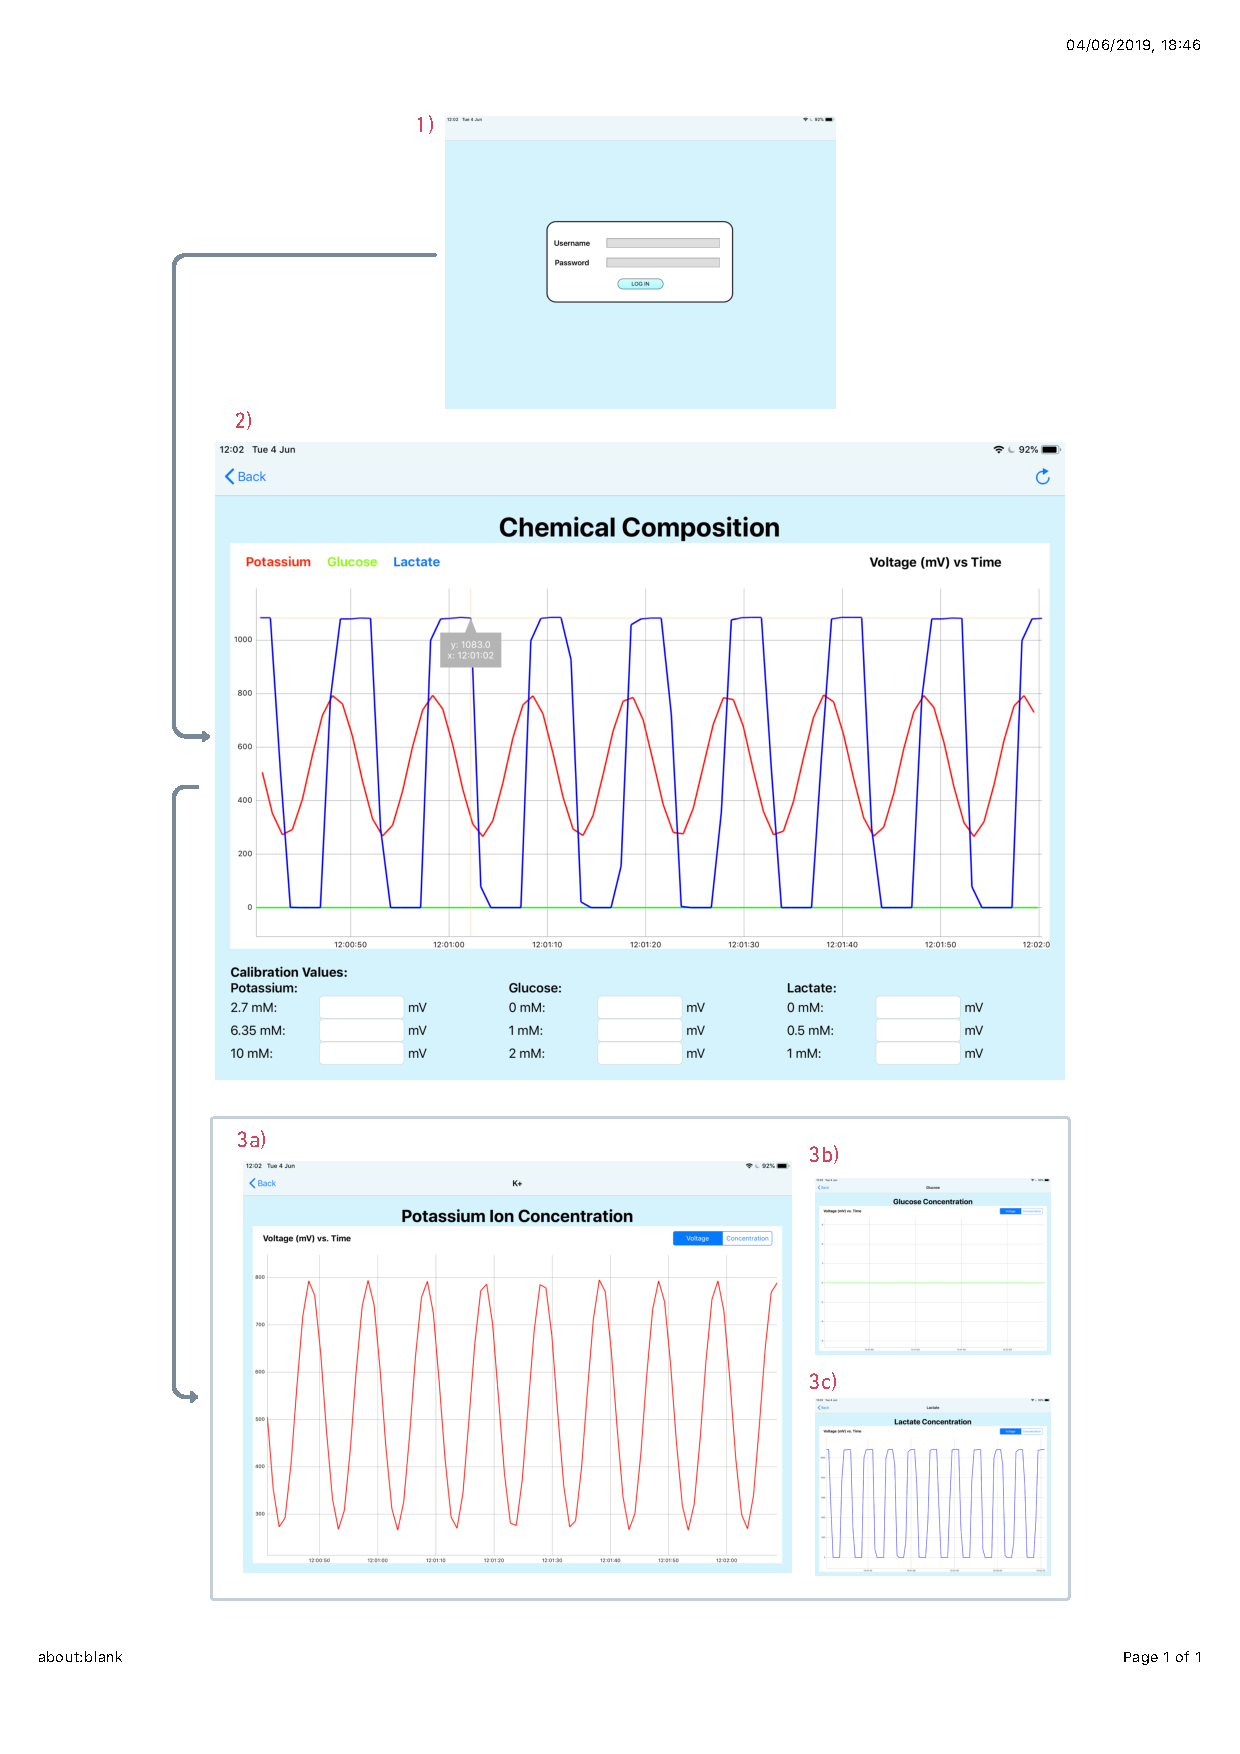
\includegraphics[trim={1cm 2.5cm 1cm  2cm}, clip, width=1\textwidth]{./figures/appStoryboard3.pdf}
\captionsetup{justification=centering}
\caption{Storyboard of the iPad application. 1) Log in page. 2) Chemical Composition page. 3a) Potassium Ion Concentration page. 3b) Glucose Concentration page. 3c) Lactate Concentration page. Pages 3a, 3b, and 3c have the same layout and are accessed from Page 2.}
\label{fig: storyboard}
\end{figure}

Once the user logs in, the app connects to and receives the strings of data sent by the Bluefruit and checks that the \textit{ID} and newline character are in place. Depending on the \textit{ID}, the app stores the \textit{Time} and \textit{Voltage} string in arrays corresponding to the electrochemical signal being read, i.e. if \textit{ID = G}, the \textit{Time} is appended to an array called  {\tt{Gtime}} and \textit{Voltage} is appended to an array called {\tt{Gvoltage}}. Each new data string for a given electrochemical signal is received every 1s. 

\subsubsection{Real Time} \label{section: real time}
The \textit{Time} string received is converted from the time (milliseconds) since the Arduino is turned on into the real clock time at which the signal was read from the Arduino analogue input pin. It is important that the signals are timestamped with the real time of recording as opposed to the time at which the signals were received on the app because there may be a lag in transmission which may vary over time.

The real time is calculated by taking the clock time at which the first input is received on the app, and subtracting the number of milliseconds encoded in the first \textit{Time} string. This provides a reference time, which is the real clock time at which the Arduino was first powered on, assuming that the delay in the first wireless transmission is negligible. Type casting is used to convert all subsequent \textit{Time} strings into doubles so that the time in milliseconds can be added to the reference time to obtain the real time at which the value was recorded on the Arduino.


\subsubsection{Charts API}
To convey the information to the clinician clearly, the data received is displayed graphically using the Charts API developed by Daniel Gindi \cite{Charts}. The API allowed for basic graphs to be fully customised based on the needs of this project. The graphs display the voltage recorded from an input pin against the real clock time of the reading for each electrochemical signal. The app allows for all three signals to be viewed on one graph, as seen on the Chemical Composition page in Figure~\ref{fig: storyboard}, or as individual plots as shown on pages 3a, 3b and 3c. These individual plots can be accessed by clicking on the graph legends on the Chemical Composition page, located above the graph. All graphs can be zoomed in and out, allowing the user to clearly view specific data. Furthermore, clicking on a specific point on a plot displays a grey bubble which shows the corresponding $x$ and $y$ values, as seen on the Chemical Composition page in Figure~\ref{fig: storyboard}.


\subsubsection{Calibration}
For the individual concentration plots on pages 3a, 3b, and 3c in Figure~\ref{fig: storyboard}, in the top right corner of the graphs there is a segmented control button that has \textit{Voltage} on the left and \textit{Concentration} on the right. Selecting a button allows the user to view the graph with either voltage or concentration on the $y$-axis. To convert the voltage values received into the corresponding concentration of the electrochemical signal in the brain, the relationship between the two needs to be known. This is obtained through calibration. 

\begin{table}[h!]
\centering
\begin{tabular}{||c c c||} 
 \hline
 [K$^{+}$] (mM) & [Glucose] (mM) & [Lactate] (mM) \\ [0.5ex] 
 \hline\hline
 2.70 & 0.00 & 0.00 \\
 6.35 & 1.00 & 0.50 \\
 10.00 & 2.00 & 1.00 \\
 \hline
\end{tabular}
\caption{Known concentrations of solutions used for calibration.}
\label{table: calibration conc}
\end{table}

The Boutelle Group have developed a novel auto-calibration system that uses programmable valves and microfluidic pumps to deliver known concentrations of potassium, glucose, and lactate, shown in Table~\ref{table: calibration conc}, to the microfluidic analysis system and the outputted voltage is recorded. Calibration occurs automatically every three hours whilst monitoring a patient because the sensors degrade over time, hence the voltage output for the same known concentration will change with time \cite{Rogers2017}. The Chemical Composition page of the app allows for the calibration values to be typed into the text field. Once inputted, the input voltages can be converted into concentration when the \textit{Concentration} button is clicked on the segmented control, and the graph displays concentration against real time. If calibration values are not provided and the \textit{Concentration} button is clicked, the app will prompt the user to insert the calibration voltages on the Chemical Composition page. 

\subsubsection{Potassium Calibration}

\begin{figure}[h!]
\centering
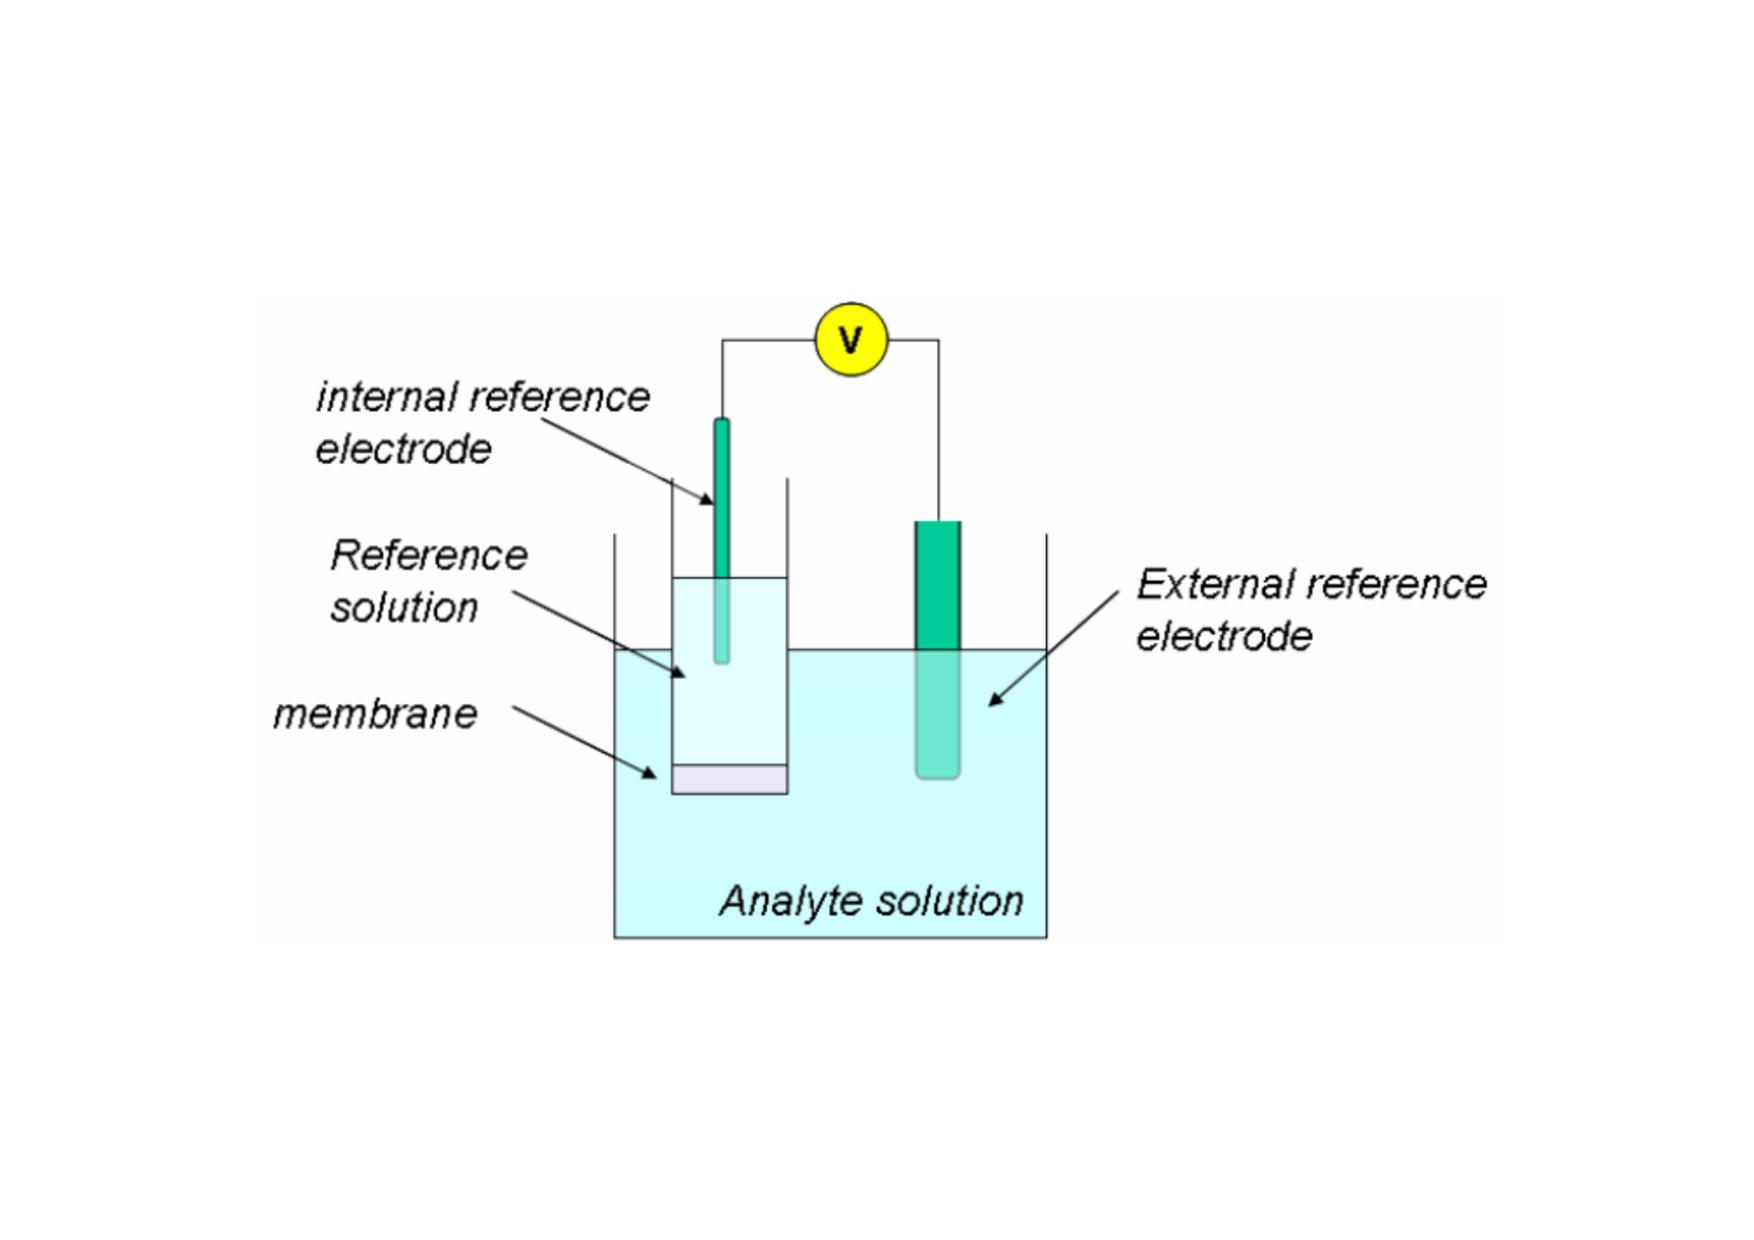
\includegraphics[trim={0cm 5cm 0cm  5cm}, clip, width=0.75\textwidth]{./figures/ISE.pdf}
\captionsetup{justification=centering}
\caption{Electrochemical cell for a potentiometric measurement with an ion selective electrode \cite{LibreTexts2019}.}
\label{fig: ISE}
\end{figure}

For potassium, the conversion from voltage to concentration is given by a logarithmic relationship and can be derived by considering the potassium sensor, which is an ion selective electrode (ISE) as shown in Figure~\ref{fig: ISE}. The ISE has an ion-sensing membrane that responds selectively to a specific ion and outputs a voltage proportional to the activity of this ion \cite{Rogers2017, LibreTexts2019} and can be derived as follows. 

The potential difference across the membrane, $E_{membrane}$ is given as the difference between the external side of the membrane, $E_{ext}$, where the analyte solution is, and the internal side of the membrane, $E_{int}$ where the reference solution is:

\begin{equation}
    E_{membrane} = E_{ext} - E_{int}.
    \label{equation: membrane potential}
\end{equation}

The potential on each side of the membrane can be described with respect to activity by using the Nernst Potential:

\begin{equation}
    E_{ext} = E^{0} + \frac{0.05916}{z}\log a_{k,ext}, 
    \label{equation: outer Nernst} 
\end{equation}
\begin{equation}
    E_{int} = E^{0} + \frac{0.05916}{z}\log a_{k,int}.
    \label{equation: inner Nernst}
\end{equation}

\noindent $E^{0}$ is the standard cell potential which is a constant, $z$ is the charge of the ion of interest which in this case is potassium so $z=1$, $a_{k,ext}$ is the activity of potassium ions in the analyte solution, and $a_{k,int}$ is the activity of the potassium ions in the reference solution which is constant. Therefore, equation (\ref{equation: inner Nernst}) is equivalent to a constant value.

Substituting equations (\ref{equation: outer Nernst}) and (\ref{equation: inner Nernst}) into equation (\ref{equation: membrane potential}), the following equation is obtained:

\begin{equation}
    E_{membrane} = constant + 0.05916\log a_{k,ext}.
    \label{equation: membrane potential 2}
\end{equation}

The relationship between activity and concentration is given as:

\begin{equation}
    a_{k,ext} = \gamma [K^{+}],
    \label{equation: activity}
\end{equation}

\noindent where $[K^{+}]$ is the concentration of potassium ions, and $\gamma$ is the activity coefficient which is approximately constant since $[K^{+}]$ is small. Taking the logarithm on both sides gives:

\begin{align}
    \log a_{k,ext} = \log\gamma + \log [K^{+}] = constant + \log [K^{+}].
    \label{equation: log activity}
\end{align}

Substituting equation (\ref{equation: log activity}) into equation (\ref{equation: membrane potential 2}) gives equation (\ref{equation: membrane potential 3}) where $C$ is a constant and $V$ is $E_{membrane}$.

\begin{equation}
    V = C + 0.05916 \log [K^{+}].
    \label{equation: membrane potential 3}
\end{equation}

\noindent Rearranging equation (\ref{equation: membrane potential 3}) gives:

\begin{equation}
    [K^{+}] = 10^{\big(\frac{V-C}{0.05916}\big)},
    \label{equation: K+ calibration}
\end{equation}

\noindent which is the equation used to convert from voltage, measured in volts, to concentration in $mM$, given that:

\begin{equation}
    C = V_{aCSF} - 0.05916\log_{10} (2.7),
    \label{equation: C}
\end{equation}

\noindent where $V_{aCSF}$ is the voltage produced by the potassium ion concentration of $2.7mM$ in the aCSF which perfuses the microdialysis probe. The aCSF is used as the reference solution. Only the voltage corresponding to $[K^{+}] = 2.7mM$ is required from the calibration set up to be substituted into equations (\ref{equation: K+ calibration}) and (\ref{equation: C}). Once the user inputs this calibration value, the user can view the concentration against time graph on the Potassium Ion Concentration page once the $Concentration$ button is clicked. \newline




\subsubsection{Glucose and Lactate Calibration}
%\noindent \underline{Glucose and Lactate Calibration} 

The conversion from voltage to concentration for glucose and lactate is derived from the enzymatic catalysed reaction that occurs on the electrode surface of the oxidase-based sensors \cite{Patel2011, Rogers2017}, and can be obtained by starting from the Hill equation. Since the sensors measure current, the Hill equation is written as

\begin{equation}
    I_{rate} = \frac{I_{max}}{1 + \big( \frac{K_{m}}{[S]} \big)^{n}},
    \label{equation: Hill equation}
\end{equation}

\noindent where $I_{rate}$ is the reaction rate, $I_{max}$ is the maximum reaction rate, $[S]$ is the substrate concentration, i.e. glucose or lactate concentration, $K_{m}$ is the substrate concentration that results in a rate that is $\frac{I_{max}}{2}$, and $n$ is the Hill coefficient which is a measure of cooperativity between the substrate and binding site.

The Hill coefficient is equal to 1 since glucose and lactate have no substrate binding cooperativity. Therefore the Hill Equation can be reduced to the Michaelis-Menten equation, which is given by:

\begin{equation}
    I_{rate} = \frac{I_{max}[S]}{[S] + K_{m}}.
    \label{equation: Michaelis_menten}
\end{equation}

Since the concentrations of glucose and lactate being measured is low, such that $[S] << K_{m}$, equation (\ref{equation: Michaelis_menten}) is reduced to a linear equation:

\begin{equation}
    I_{rate} = \frac{I_{max}[S]}{K_{m}}.
    \label{equation: reduced Michaelis_menten}
\end{equation}

\noindent Since the transimpedance amplifier converts the current to voltage, the relationship between voltage and concentration is linear in the form of $y = mx + c$.

During calibration, only three known concentrations of solutions are used and the corresponding voltages recorded. Having few data points reduces the accuracy of the linear equation that best fits through the data points. Furthermore, there are numerous lines of best fit that would fit the data. The optimal line of best fit can be found using least squares regression:

\begin{equation}
    m = \frac{ \sum_{i=1}^{3} \big( x_{i} - \Bar{X} \big) \big( y_{i} - \Bar{Y} \big) }{ \sum_{i=1}^{3} \big( x_{i} - \Bar{X} \big)^{2} },
    \label{equation: least squares regression}
\end{equation}
\begin{equation}
    c = \Bar{Y} - m\Bar{X},
\end{equation}

\noindent where $x_{i}$ is the voltage recording, $\Bar{X}$ is the mean voltage recording, $y_i$ is the known concentration, and $\Bar{Y}$ is the mean concentration from the data set of known concentrations. 

Now that the $m$ and $c$ coefficients have been determined, the plot of voltage against time can be transposed into concentration against time for glucose and lactate using $Concentration = m \times Voltage + c$.


